\section{Theory and Methods}

\subsection{Heat Equation and Problem Domain}

From the final project assignment:
The heat equation is solved on a disk $\Omega$ with the boundary $\Gamma$ (\refFig{fig::Domain}) to obtain the radial temperature distribution. The Problem is given by the following heat equation, using Dirichlet boundary conditions at the disk outer boundary and an initial homogeneous Temperature $T_0$ on the whole disk:
\begin{align}
	\label{eq:Heat}
	\pp{T}{t}-\kappa \nabla^2 T &= f &&\text{on} \ \Omega \ \forall t \in (0,t_f),\\
	T(\vect{x},t) &= T_D &&\text{on} \ \Gamma \ \forall t \in (0,t_f), \label{eq:Dirichlet}\\
	T(\vect{x},0) &= T_0 &&\text{on} \ \Omega.
\end{align}
where $T$ is the temperature, $\kappa$ the thermal diffusivity, and $f$ the thermal heat source. The problem is solved for the time interval $t \in (0,t_f)$, with the final solution time $t_f$. The heat source is a function of the radius of the plate with:
\begin{equation}
	f(r) = \left\{\begin{array}{ll}\frac{Q}{\pi R_1^2} & \text{if} \ r < R_1, \\
		0 & \text{if} \ r \geq R_1 \end{array}\right . .
\end{equation}
where $Q=P \cdot d_z$ is the volumetric heat source and $d_z = 0.1m $ the out-of-plane thickness. For validation purposes an analytical solution for $t \rightarrow \infty$ is given by:
\begin{equation}
	\label{eq:analytical}
	T(r) = \left\{\begin{array}{ll} T_0-\frac{Q}{2 \pi \kappa } \big(\frac{1}{2} \big(\frac{r^2}{R_1^2} - 1\big)\big)+ln\big(\frac{R_1}{R_2}\big) & \text{if} \ r < R_1, \\
		T_0 - \frac{Q}{2 \pi \kappa } ln\big(\frac{r}{R_2}\big)& \text{if} \ r \geq R_1 \end{array}\right . .
\end{equation}
The parameters for the specific heated disk problem are provided in \refTab{tab:parameters}.
\begin{figure}[h!]
	\centering
	\resizebox{0.6\width}{!}{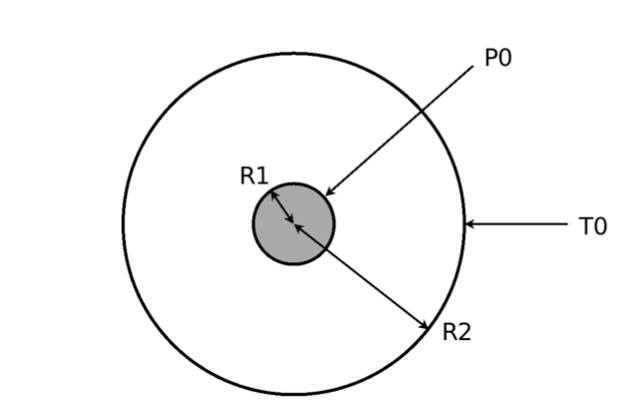
\includegraphics{plots/Problem_domain.png}}
	\caption{\label{fig::Domain} Problem domain}
\end{figure}

\renewcommand{\arraystretch}{2}
\begin{table}[h!]
	\begin{center}
		\begin{tabular}{ p{5cm} p{2cm} p{1.5cm} p{1.5cm}}
			\toprule
			Parameter & Variable & Value & Unit\\
			\hline
			Inner circle radius & $R_1$ & 0.01 & $[m]$\\
			Outer circle radius & $R_2$ & 0.1 & $[m]$\\
			Heat source on the area & $Q$ & 100 & $[W]$\\
			Dirichlet BC temperature & $T_0(x,y)$ & 500 & $[K]$\\
			Initial temperature & $T_s(x,y,0)$ & 0 & $[K]$\\
			Thermal diffusivity & $\kappa$ & 1.0 & $[m^2/s]$\\
			\bottomrule
		\end{tabular}
		\caption{\label{tab:parameters} Problem parameters for the heated disk problem}
	\end{center}
\end{table}
\renewcommand{\arraystretch}{1}

\subsection{Weak Form}

To obtain a discrete formulation in space and time for a finite element discretization for the unsteady heat equation, a weak or variational form of \refEq{eq:Heat} has to be defined. Two sets of function spaces have to be defined in the context of the standard Galerkin formulation \cite{doneaFiniteElementMethods2003}:
\begin{align}
	\mathcal{V} &= \{w \in \mathcal{H}^1(\Omega) | w = 0 \text{ on } \Gamma_D\}\\
	\mathcal{S} &= \{T \in \mathcal{H}^1(\Omega) | T = T_D \text{ on } \Gamma_D\}
\end{align}
where the space $\mathcal{V}$ is composed of test functions that are square integrable and have square integrable first derivatives over the computational domain $\Omega$. They vanish on the Dirichlet boundary $\Gamma_D$. The set of functions $\mathcal{S}$ are the trial solutions. This collection of functions has similar properties to the test functions, except that those functions have to satisfy the Dirichlet boundary condition on the domain boundary $\Gamma_D$. $\mathcal{S}$ and $\mathcal{V}$ are both continuous function spaces. For the finite element method these function spaces are approximated by finite dimensional subsets $\mathcal{S}^h$ and $\mathcal{V}^h$.

The weak formulation of \refEq{eq:Heat} is given as:
\begin{equation}
	\label{eq:weak}
	\int_{\Omega} w\pp{T}{t} d\Omega - \kappa \int_{\Omega} w \nabla^2 T d\Omega = \int_{\Omega}w f d\Omega \ \ \forall w .
\end{equation}
By applying the Green-Gauss divergence theorem on the left-hand-side (LHS) of \refEq{eq:weak}, the order of the spatial derivatives can be reduced. Together with a zero homogeneous Neumann boundary condition ($n \cdot \nabla T = 0 \text{ on } \Gamma_h$), we obtain the following equation:
\begin{equation}
	\label{eq:weak2}
	\int_{\Omega}w\pp{T}{t} d\Omega + \kappa \int_{\Omega} \nabla w \cdot \nabla T d\Omega = \int_{\Omega} w f d\Omega
\end{equation}

\subsection{Finite Element Method}

The discretized variational formulation of the continuous PDE in weak form (\refEq{eq:weak2})  that is used for the FEM, is formulated as: find $T^h \in \mathcal{S}^h$, such that $\forall w^h \in \mathcal{V}^h$

\begin{equation}
	\sum_{B \in \eta \backslash \eta_D} \Bigg[(N_A,N_B) \pp{T_b}{t} + a(N_A,N_B)T_B \Bigg] = (N_A,f) - \sum_{B \in \eta_D} a(N_A,N_B)T_D(\vect{x}_B), \forall A \in \eta \backslash \eta_D .
\end{equation}
with
\begin{equation}
	T^h(\vect{x}) = \sum_{B\in \eta}N_B(\vect{x})T_B ,
\end{equation}
where $N_A$ are the shape functions used for the interpolation of the continuous weighting function $w(x,y)$, $N_B$ are the shape functions for the interpolation of $T(x,y)$, $a(N_A, N_B)$ represents the discretized thermal diffusive part of the equation (second term on left-hand-side in \refEq{eq:weak2}) and $(N_A,f)$ denotes the discretized version of the right-hand-side. $\eta$ represents the set of all nodes and $\eta_D$ is a subset of $\eta$ containing all nodes on the boundary, where the Dirichlet boundary condition is applied.

This variational formulation leads to a matrix form of equations:
\begin{equation}
	[M] \Big\{ \dot{T} \Big\} + [K] \Big\{ T \Big\} = \Big\{ F \Big\} 
\end{equation}
where $M$ refers to the mass matrix, $K$ to the stiffness matrix and $F$ to the source vector. After applying a first order explicit time integration scheme and isolating the LHS by inverting the mass matrix $M$ the explicit equation to obtain the temperature at the nodes for a time step $n$ can be written as:
\begin{equation}
	\label{eq:LHS}
	\{T\}^{n+1} = ([M]^n)^{-1}([M]^n\{T\}^n + \Delta t(\{F\}^n-[K]^n\{T\}^n)
\end{equation}

In a first step the mass matrices are computed on element level and then assembled globally. To solve the integrals efficiently in combination with the unstructured grid, an isoparametric approach is chosen. Therefore, the integrals are evaluated on a triangular reference element. To map the results back to the physical domain, the transformation theorem is applied:
\begin{equation}
	\int_{\Omega^e} \Phi(\vect{x}) d\vect{x} = \int_{\Omega^{ref}} \Phi(\xi, \eta)) |\vect{J}(\xi, \eta)| d\xi d\eta 
\end{equation}
$\Phi$ denotes an arbitrary function in $\mathcal{S}$, $\vect{J}$ the Jacobian for the transformation between global coordinates ($x,y$) and the reference coordinates $(\xi, \eta)$, $\Omega^e$ the physical element domain and $\Omega^{ref}$ the reference domain of the element. The integrals are solved numerically by using Gaussian quadrature:
\begin{equation}
	\int_0^1 \int_{0}^{1-\eta} \Phi(\xi, \eta) d\xi d\eta \approx \sum_{i=1}^{n_{quad}} w_i \Phi(\xi_i, \eta_i)
\end{equation}
with weights $w_i$ and $\xi_i, \eta_i$, the quadrature points at which $\Phi(\xi, \eta)$ is determined. The individual entries of the matrices $M,K$ and $F$ are then calculated as follows:
\begin{align}
	M_{i,j}^e &= \sum_{m=1}^{n_{quad}}w(m) S_i(\xi_m \eta_m)S_j(\xi_m, \eta_m) | \vect{J}_m | , \label{eq:M} \\ 
	K_{i,j}^e &= \kappa \sum_{m=1}^{n_{quad}}w(m) (\partial_x S_i(\xi_m, \eta_m)) \partial_x S_j(\xi_m, \eta_m) + 
	\partial_y S_i(\xi_m, \eta_m) \partial_y S_j(\xi_m, \eta_m) | \vect{J}_m | , \label{eq:K} \\
	F_i^e &=  \sum_{m=1}^{n_{quad}} w(m) f S_i(\xi_m, \eta_m) | \vect{J}_m |. \label{eq:F}
 \end{align}
For an efficient inversion of the mass matrix, which is necessary to obtain the spacial temperature distribution for the next time step (\refEq{eq:LHS}), mass lumping is used. This technique is an approximation of the original system, transforming the mass matrix into a diagonal matrix, which can be stored as a vector.
\newpage

\subsection{Meshes}
For the FEM Solver, three different unstructured meshes are used with different refinement levels (coarse, medium and fine). The number of nodes and elements of the three different unstructured triangular meshes (coarse, medium and fine) are presented in \refTab{tab:Mesh}.
\renewcommand{\arraystretch}{2}
\begin{table}[h!]
	\begin{center}
		\begin{tabular}{ p{2cm} p{1.5cm} p{1.5cm} }
			\hline
			\hline
			mesh & number nodes (nn) & number elements (ne)\\
			\hline
			coarse & 2041 & 3952\\
			\hline
			medium & 21650 & 21332\\
			\hline
			fine & 85290 & 84656\\
			\hline
			\hline
		\end{tabular}
		\caption{\label{tab:Mesh} Number of nodes and elements for the three different meshes}
	\end{center}
\end{table}
\renewcommand{\arraystretch}{1}